\documentclass[12pt,a4paper]{article}
\usepackage[utf8]{inputenc}
\usepackage{amsmath}
\usepackage{amsfonts}
\usepackage{amssymb}
\usepackage{graphicx}
\usepackage{tikz}
\usepackage{pgfplots}
\usepackage[left=2cm,right=2cm,top=2cm,bottom=2cm]{geometry}
\author{\LARGE Amin Gamil}
\title{{\huge \textsc{Task 5.2 – ADC}}}
\date{}
\begin{document}
\maketitle

\section{3-bit encoder with Sampling Time = 0.25sec}
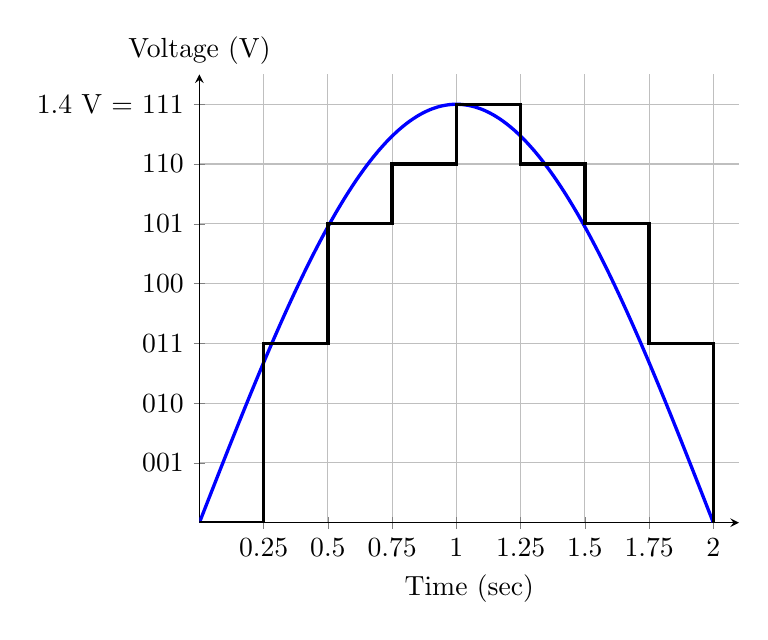
\begin{tikzpicture}
\begin{axis}[
    axis lines = center,
    xlabel = {Time (sec)},
    ylabel = {Voltage (V)},
    xlabel near ticks,
 %   xlabel style={center},
  	ylabel style={above},
    xtick={0,0.25,...,2},
    ytick={0,0.2,...,1.4},
    ymax = 1.5,
    ymin = 0,
    xmin = 0,
    xmax = 2.1,
   yticklabels = {
   000,
   {001},
   010,
   011,
   100,
   101,
   110,
   {1.4 V = 111},},
   xmajorgrids=true,
   ymajorgrids=true,
%    width=2.5cm,
%    height=1cm,
%    scale only axis,
]
\addplot [
	very thick,
    color=blue,
    smooth,
    domain=0:2,
    samples=50,
]
{1.4*sin(deg(pi*x/2))};


\addplot [
	very thick,
    color=black,
    domain=0:2,
    samples=50,
]
coordinates
{(0,0)(0,0)(0.25,0)
(0.25,0.6)(0.5,0.6)
(0.5,1.0)(0.75,1.0)
(0.75,1.2)(1,1.2)
(1,1.4)(1.25,1.4)
(1.25,1.2)(1.5,1.2)
(1.5,1.0)(1.75,1.0)
(1.75,0.6)(2,0.6)(2,0)
};
\end{axis}
\end{tikzpicture}\\
Digital sequence = 000 011 101 110 111 110 101 011

\section{3-bit encoder with Sampling Time = 0.5sec}
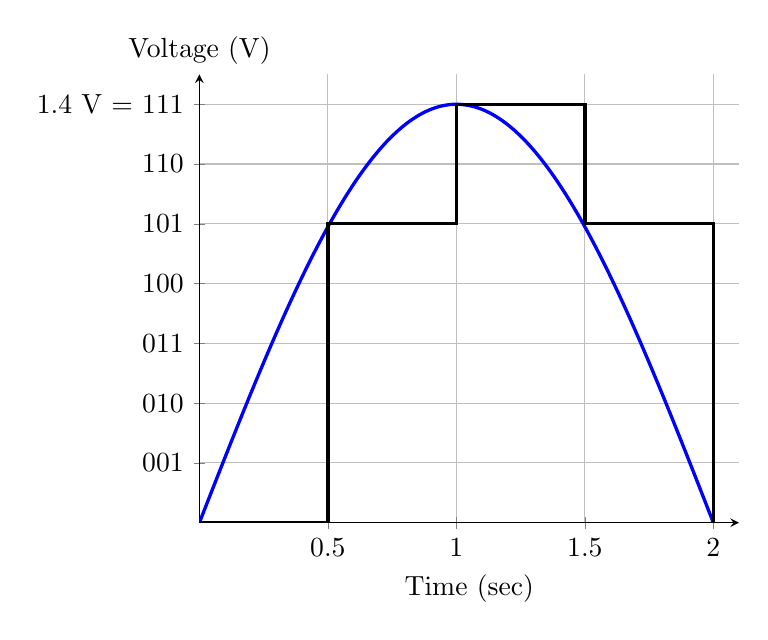
\begin{tikzpicture}
\begin{axis}[
    axis lines = center,
    xlabel = {Time (sec)},
    ylabel = {Voltage (V)},
    xlabel near ticks,
 %   xlabel style={center},
  	ylabel style={above},
    xtick={0,0.5,...,2},
    ytick={0,0.2,...,1.4},
    ymax = 1.5,
    ymin = 0,
    xmin = 0,
    xmax = 2.1,
   yticklabels = {
   000,
   {001},
   010,
   011,
   100,
   101,
   110,
   {1.4 V = 111},},
   xmajorgrids=true,
   ymajorgrids=true,
%    width=2.5cm,
%    height=1cm,
%    scale only axis,
]
\addplot [
	very thick,
    color=blue,
    smooth,
    domain=0:2,
    samples=50,
]
{1.4*sin(deg(pi*x/2))};


\addplot [
	very thick,
    color=black,
    domain=0:2,
    samples=50,
]
coordinates
{(0,0)(0.5,0)
(0.5,1.0)(1,1)
(1,1.4)(1.5,1.4)
(1.5,1.0)(2,1.0)(2,0)
};
\end{axis}
\end{tikzpicture}\\
Digital sequence = 000 101 111 101

\section{3-bit encoder with Sampling Time = 1sec}
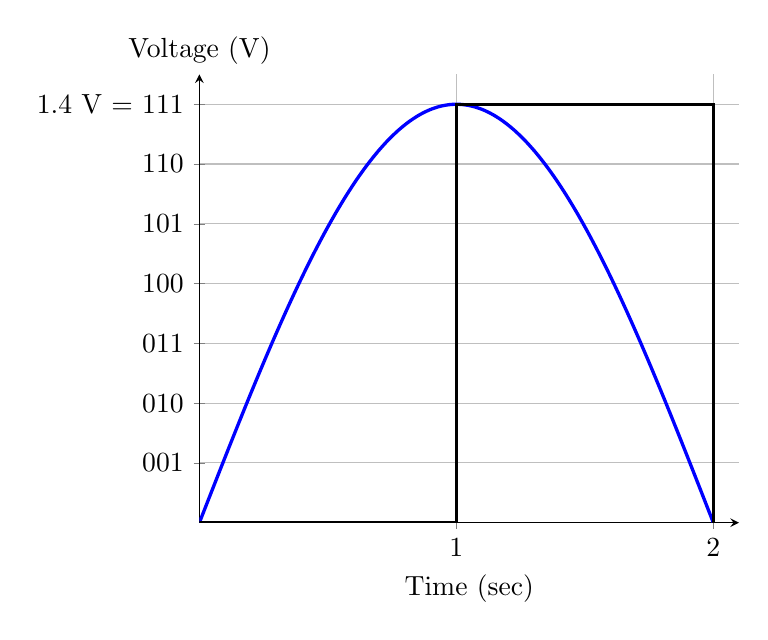
\begin{tikzpicture}
\begin{axis}[
    axis lines = center,
    xlabel = {Time (sec)},
    ylabel = {Voltage (V)},
    xlabel near ticks,
 %   xlabel style={center},
  	ylabel style={above},
    xtick={0,1,...,2},
    ytick={0,0.2,...,1.4},
    ymax = 1.5,
    ymin = 0,
    xmin = 0,
    xmax = 2.1,
   yticklabels = {
   000,
   {001},
   010,
   011,
   100,
   101,
   110,
   {1.4 V = 111},},
   xmajorgrids=true,
   ymajorgrids=true,
%    width=2.5cm,
%    height=1cm,
%    scale only axis,
]
\addplot [
	very thick,
    color=blue,
    smooth,
    domain=0:2,
    samples=50,
]
{1.4*sin(deg(pi*x/2))};


\addplot [
	very thick,
    color=black,
    domain=0:2,
    samples=50,
]
coordinates
{(0,0)(1,0)(1,1.4)
(2,1.4)(2,0)

};
\end{axis}
\end{tikzpicture}\\
Digital sequence = 000 111

\section{2-bit encoder with Sampling Time = 0.25sec}
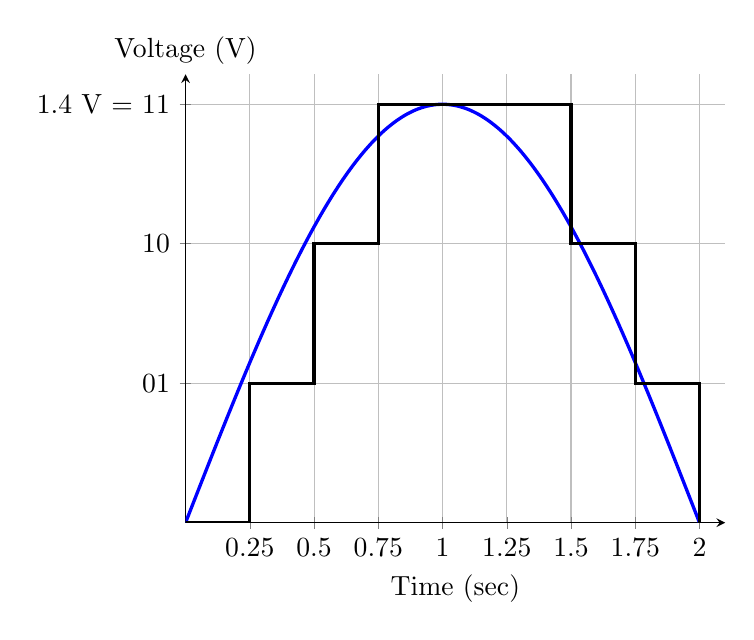
\begin{tikzpicture}
\begin{axis}[
    axis lines = center,
    xlabel = {Time (sec)},
    ylabel = {Voltage (V)},
    xlabel near ticks,
 %   xlabel style={center},
  	ylabel style={above},
    xtick={0,0.25,...,2},
    ytick={0,1.4/3,...,1.4},
    ymax = 1.5,
    ymin = 0,
    xmin = 0,
    xmax = 2.1,
   yticklabels = {
   00,
   01,
   10,
   {1.4 V = 11},},
   xmajorgrids=true,
   ymajorgrids=true,
%    width=2.5cm,
%    height=1cm,
%    scale only axis,
]
\addplot [
	very thick,
    color=blue,
    smooth,
    domain=0:2,
    samples=50,
]
{1.4*sin(deg(pi*x/2))};


\addplot [
	very thick,
    color=black,
    domain=0:2,
    samples=50,
]
coordinates
{(0,0)(0.25,0)(0.25,1.4/3)
(0.5,1.4/3)(0.5,1.4/3*2)
(0.75,1.4/3*2)(0.75,1.4)
(1.25,1.4)(1.25,1.4)(1.5,1.4)(1.5,1.4/3*2)
(1.75,1.4/3*2)(1.75,1.4/3)(2,1.4/3)(2,0)

};
\end{axis}
\end{tikzpicture}\\
Digital sequence = 00 01 10 11 11 11 10 01


\end{document}